Quello che vogliamo fare ora è passare partendo da un simbolo distinto espandendo una serie di regole per cui alla fine del processo avrò la parola.
L'altro processo è l'opposto parto dalla parola e cerco di capire quali sono gli ultimi pezzi che hanno composto la parola e poi proceso all'indietro fino ad arrivare al simbolo distinto, in questo modo cerco di riaggregare i pezzi andando dal basso verso l'alto.
Questi a grandi linee sono le due strategie che applicheremo per il parsing. I due modi si chiamano:
\begin{enumerate}
    \item \textbf{Top-down}: Parto dal simbolo distinto e cerco di arrivare alla parola
    \item \textbf{Bottom-up}: Parto dalla parola e cerco di arrivare al simbolo distinto
\end{enumerate}

Notiamo che questi approcci possono essere appliacati a tutte le grammatice, ad esempio vediamo una grammatica context sensitive, nel caso top down:
\begin{lstlisting}
w = 'aabbcc'

G = Grammar.from_string("""
S -> a S Q | a b c
b Q c -> b b c c  
c Q -> Q c
""", False)

steps = (0, 0), (1, 1), (3, 3), (2, 2)

for nprod, pos in steps: print(pos, G.P[nprod])

\end{lstlisting}

Nel caso bottom up quello che a volte conviene fare è ribaltare la grammatica, le produzioni left producono le right, questo ovviamente va a rovinare la nostra grammatica, poi possiamo mettere anche un simbolo Inizio e Fine per indicare l'inizio e la fine della produzione. Spesso lavorando in questo modo si produce una derivazione right-most (sostituisco il simbolo più a destra della derivazione non sentenziale e sostanzialmente faccio i passi da destra a sinistra dall'ultimo al primo). Posso decidere dall'alto in basso e queso produce derivazioni left-most oppure posso andare dal basso verso l'alto cercando di aggregare e ottengo derivazioni right-most ma che devo leggere dal basso verso l'alto.

\begin{lstlisting}
GR = Grammar.from_string("""
Inizio -> a a b b c c
a S Q -> S
a b c -> S 
b b c c -> b Q c
Q c -> c Q
S -> Fine
""", False)

steps = (0, 0), (3, 2), (4, 3), (2, 1), (1, 0), (5, 0)

for nprod, pos in steps: print(pos, GR.P[nprod])
\end{lstlisting}

\section{NPDA}
In realtà questo tipo di comportamento viene modellato nell'ambito del parsing attraverso la nozione di automa che ha bisogno di un nastro di input ed un area di memoria per tenere il processo di parsing, sostanzialmente deve fare la scansinoe della parola e mano a mano costruire l'albero di derivazione. Tutti gli algoritmi che vedremo hanno bisogno di una pila (stack) come forma di memoria per tenere traccia del processo di parsing perchè il tipo di lavoro che fanno non richiede un accesso causale alla memoria. Ma come fanno a decidere questi automi? hanno un dispositivo di controllo che è in grado di determinare cosa fare, come spostarsi sul nastro e cosa scrivere e prendere dalla pila. La cosa più intuitiva che uno può fare è avere una mente omiscente che è in grado di determinare cosa l'automa in ogni situazione deve fare. Quello che dovremo fare nel nostro lavoro è costruire questo controllo e poi trovare un modo per elminare il non determinismo perchè non avremo l'oracolo che sa tutto.

Quello che accadrà è che data una descrizione della grammatica sarà possibile realizzare la struttura di controllo dell'automa in maniera automatica, potremmo pensare ad un programma che dato in pasto la grammatica G produca l'automa, questi programmi si chiamano \underline{parser generator}.
Un'altro modo molto usuale, che descrive una grande famiglia di algoritmi di parsing, è quello di avere un controllo universale (che funziona per ogni grammatica) trasformando una tabella che rappresenta le informazioni che G contiene in una forma che fa in modo che il controllo sappia cosa fare, questo metodo si chiama \underline{table driven}.

Nell'analizzare il comportamento di questi parser ci sono due grandezze che vogliamo vedere:
\begin{enumerate}
    \item Lo spazio in memoria, quanto spazio consuma l'automa nel funzionamento sempre in rapporto alla lunghezza della parola
    \item Il tempo di esecuzione, quanto tempo impiega l'automa a processare la parola
\end{enumerate}

Evidente più è alto il tipo di grammatica più è alta la memoria e più scendiamo il contrario.
Noi ci occuperemo delle context-free e per quel che concerne gli altri due livelli della gerarchia osserviamo questo:
\begin{itemize}
    \item Le tipo 0 (unrestricted) rappresentano gli insiemi ricorsivamente enumerabili, quindi chiedersi se una parola appartiene ad una grammatica di tipo 0 equeivale a chiedersi se il programma termina, problema indecidibile
    \item Le tipo 1 (context sensitive) sono più deboli delle unrestricted, sono gli insiemi accettati da una macchina di Turing non deterministica, problema decidibile ma non in tempo polinomiale bensì in tempo e spazio esponenziale. Questo è il livello in cui si colloca il parsing naturale (linguaggi naturali).
    \item Le tipo 2 (context free) sono gli insiemi accettati da un NPDA, problema decidibile in tempo polinomiale.
\end{itemize}

Una cosa che vale la pena considerare nell'ambito del parsing context-free esiste una possibile divisione del lavoro che dobbiamo fare raggruppando sulla base di qualche criterio. Una prima grande dicotomia è se gli algoritmi funzionano in maniera:
\begin{enumerate}
    \item top-down
    \item bottom-up
\end{enumerate}

Un'altra dicotomia piuttosto interessante è il modo in cui l'input viene analizzato, perchè l'automa può andare avanti ed indietro nell'input:
\begin{enumerate}
    \item Parser direzionale: L'automa va avanti e indietro nell'input, in ordine, se lo ciuccia man mano che riceve i byte
    \item Parse non direzionale: il parser può adoperare delle porzioni del nastro diverse, ad esempio nell'uso degli editor abbiamo la colorizzazione della sintassi, in questo caso il parser non è direzionale perchè se fosse direzionale dovrei ricostruire tutto l'albero per ogni modifica.
\end{enumerate}

Un'altra possibile dicotomia che abbiamo già in qualche modo accennato è il fatto che purtroppo abbiamo il non determinismo e per risolvere questo potrebbe provare tutti i passi agendo:
\begin{enumerate}
    \item Depth first
    \item Breadth first
\end{enumerate}

Una possibilità cruciali per eleminare il problema del non determinismo è avere un parsing che a priori non accetti qualsiasi grammatica ma solo quelle che sono in una certa forma, quelle deterministiche (si rispippola la grammatica in modo che sia deterministica). Questo ci crea dei parsing molto meno potenti.

Cosa vedermo noi:
\begin{enumerate}
    \item Non directional methods Bottom-up: CYK parser
    \item Deterministic directional:
    \begin{enumerate}
        \item Top-down: LL parser, mescolare parsing e traduzione è più semplice dell LR. Sono meno efficienti ma pace, noi useremo un parser generator LL(*). Noi vedremo LL(1).
        \item Bottom-up: LR parser, vedremo LR(0)
    \end{enumerate}
\end{enumerate}

\section{CYK parser}
L'algoritmo CYK si basa su una tabella che rappresenta la comprensione temporanea che ha l'algoritmo del processo di parsing (della costruzione dell'albero di parsing) e questa tabella più essere facilmente riempita nel caso in cui la grammatica abbia una forma semplificata che per il momento noi assumeremo. Le regole che vorremo avranno solo questa forma, una produzione non terminale o di una coppia:
\begin{lstlisting}
    A -> BC
    A -> a
\end{lstlisting}

La tabella di questo algoritmo è fatta così, sulla base abbiamo la parola e poi ha una serie di celle in cui in ciascuna cella contiene l'informazione della sotto-parola la cui lunghezza è data dalla riga in cui mi trovo e che raccontano l'idea che si è fatto l'algoritmo di parsing della stringa lunga due a partire dalla posizione della tabella sotto. Nella posizione i,l rappresenta l'informazione che ho sul parsing del prefisso della parola che comincia lì ed è lunga l:
\begin{lstlisting}
INPUT = 'unaprova'

n = len(INPUT)

R = CYKTable()
for l in range(1, n + 1):
  for i in range(1, n - l + 2): 
    R[i, l] = INPUT[(i) - 1: (i + l) - 1]
\end{lstlisting}

\begin{figure}[ht!]
  \centering
  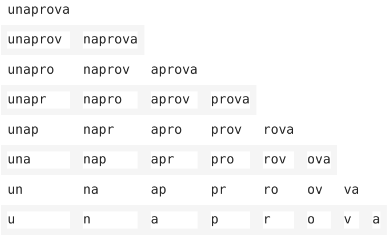
\includegraphics[scale=1]{images/Parsing/tabellaR.png}
\end{figure}


Osserviamo che la tabelle può essere riempita in due modi, siccome ogni posizione riguarda un sottoinsieme la posso riempire in due modi:
\begin{enumerate}
    \item offline: parto dal fondo a sinistra e comincio a mettere le lettere singole, poi sopra le coppie e così visita. Offline perchè per riempirla devo aver visto tutto l'input
    \item online: la riempio in diagonale partendo dal basso a sinistra, mano mano che vedo caratteri posso riempire sempre più celle
\end{enumerate}

\begin{lstlisting}
 def offline(fill, n):
  R = CYKTable()
  for l in range(1, n + 1):
    for i in range(1, n - l + 2): 
      R[i, l] = fill(R, i, l)
  return R 

def online(fill, n):
  R = CYKTable()
  for d in range(1, n + 1):
    for i in range(d, 0, -1):
      R[i, d - i + 1] = fill(R, i, d - i + 1)
  return R
\end{lstlisting}

Noi ovviamente non la riempiremo di parti di parola ma di produzioni, per filtrare le produzioni useremo la funzione di python filter che filtra cose in base ad una funzione che gli passiamo.
Quando siamo in alto nella tabella dobbiamo mettere una produzione che da A produce BC, perchè vogliamo metterci qualcosa che produce quello che c'è sotto quindi sotto dobbiamo andare a vedere se B produce un pezzo di quello che c'è sotto e la C il resto.

In buona sostanza se sono a lunghezza 1 ci metto tutti i terminali dove A produce a dove a è proprio la parola (lettera negli esempi) che sto cercando, se sono a lunghezza 2 metto tutte le produzioni che producono due terminali B e C dove B produce la parola da i a k e c da k in poi.
\begin{lstlisting}
 def cyk_fill(G, INPUT):
  def fill(R, i, l):
    res = set()
    if l == 1:
      for A, (a,) in filter(Production.such_that(rhs_len = 1), G.P): 
        if a == INPUT[i - 1]: res.add(A)
    else:
      for k in range(1, l):
        for A, (B, C) in filter(Production.such_that(rhs_len = 2), G.P):
          if B in R[i, k] and C in R[i + k, l - k]: res.add(A)
    return res
  return fill
\end{lstlisting}

Vediamo degli esempi su una grammatica $a^n$:
\begin{lstlisting}
G = Grammar.from_string("""
S -> A S
A -> a
S -> .
""")

INPUT = 'aaa.'

online(cyk_fill(G, INPUT), len(INPUT))
\end{lstlisting}

\begin{figure}[ht!]
  \centering
  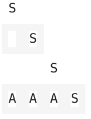
\includegraphics[scale=1]{images/Parsing/tabellaRes1.png}
\end{figure}

\begin{lstlisting}
 INPUT = 'aa.a.'

online(cyk_fill(G, INPUT), len(INPUT))
\end{lstlisting}

\begin{figure}[ht!]
  \centering
  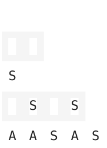
\includegraphics[scale=1]{images/Parsing/tabellaRes2.png}
\end{figure}

\begin{lstlisting}
# fig. 4.15, pag. 123 

G = Grammar.from_string("""
Number -> 0|1|2|3|4|5|6|7|8|9 
Number -> Integer Digit
Number -> N1 Scale' | Integer Fraction
N1 -> Integer Fraction
Integer -> 0|1|2|3|4|5|6|7|8|9 
Integer -> Integer Digit
Fraction -> T1 Integer
T1 -> .
Scale' -> N2 Integer
N2 -> T2 Sign
T2 -> e
Digit -> 0|1|2|3|4|5|6|7|8|9 
Sign -> + | -
""")
\end{lstlisting}

\begin{figure}[ht!]
  \centering
  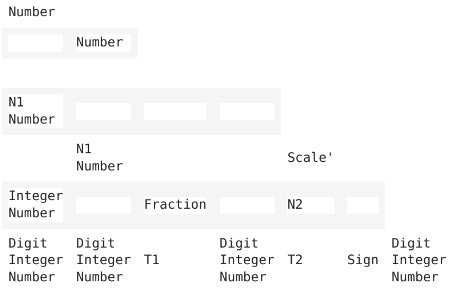
\includegraphics[scale=1]{images/Parsing/tabellaResComplesso.png}
\end{figure}


Negli esempi si vede bene che sotto mettiamo tutti i terminali delle produzioni a sinistra che producono la parola o lettera (ad esempio A produce a quindi ci metto A per tutte le volte che ci sono a nella parola). Poi per le celle sopra ci chiediamo se c'è una produzione che produce $A \rightarrow BC$ dove B produce la sotto parola da i a k e C da k in poi (ad esempio $S \rightarrow A, S$).

Per guardare se la parola fa parte del linguaggio basta guardare la cella in alto della tabella, se è riempita significa che è ok.
\subsection{Albero di parsing}
Dobbiamo ricostruire l'albero di parsing da questa tabella, al momento ci accontentiamo di costurire l'albero i cui nodi sono i non terminali e gli archi le produzioni (non ha dentro le produzioni). Non è super difficile perchè possiamo approcciare questa cosa ricorsviamente.
Scriviamo una funzione ricorsiva fake\_parse che (usando la tabella R, la grammatica G e l'input INPUT) dato un non terminale, il punto d'inizio e la lunghezza, restituisca l'albero di parsing radicato in quel non terminale e che deriva la sottostringa specificata.

\begin{lstlisting}
def cyk_fill(G, INPUT):
  def fill(R, i, l):
    res = set()
    if l == 1:
      for A, (a,) in filter(Production.such_that(rhs_len = 1), G.P): 
        if a == INPUT[i - 1]: res.add(A)
    else:
      for k in range(1, l):
        for A, (B, C) in filter(Production.such_that(rhs_len = 2), G.P):
          if B in R[i, k] and C in R[i + k, l - k]: res.add(A)
    return res
  return fill
\end{lstlisting}

\begin{figure}[ht!]
  \centering
  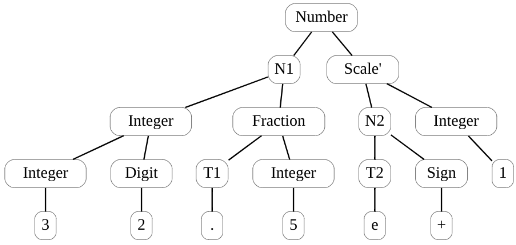
\includegraphics[scale=1]{images/Parsing/fake_parser.png}
\end{figure}

\subsection{Riduzione in forma normale di Chomsky}
La forma normale di Chomsky è una forma normale in cui tutte le produzioni sono della forma:
\begin{lstlisting}
    A -> BC
    A -> a
\end{lstlisting}

Per ottenere una grammatica in forma normale di Chomsky dobbiamo fare due passaggi:
\begin{enumerate}
    \item Eliminare le regole unitarie
    \item Eliminare le produzioni più lunghe di 2, riduzione in forma normale, trasformazioni produzione non solitarie
    \item Eliminare le epsilon regole
\end{enumerate}

\begin{lstlisting}
def remove_unproductive_unreachable(G):
  def find_productive(G):
    @closure
    def find(prod):
      return prod | {A for A, a in G.P if set(a) <= prod}
    return find(G.T)
  def find_reachable(G):
    @closure
    def find(reach):
      return reach | union_of(set(a) for A, a in G.P if A in reach)
    return find({G.S})
  Gp = G.restrict_to(find_productive(G))
  return Gp.restrict_to(find_reachable(Gp))

def cyk(G, INPUT):
  def fill(R, i, l):
    res = set()
    if l == 1:
      for A, (a,) in filter(Production.such_that(rhs_len = 1), G.P): 
        if a == INPUT[i - 1]: res.add(A)
    else:
      for k in range(1, l):
        for A, (B, C) in filter(Production.such_that(rhs_len = 2), G.P):
          if B in R[i, k] and C in R[i + k, l - k]: res.add(A)
    return res
  R = CYKTable()
  for l in range(1, len(INPUT) + 1):
    for i in range(1, len(INPUT) - l + 2):
      R[i, l] = fill(R, i, l)
  return R
\end{lstlisting}


\subsection{Elminazione epsilon-regole}
Una epsilon regola è una regola della forma A -> $\epsilon$, cioè una regola che produce la parola vuota.
Per eleminare una epsilon regola poteri duplicare la regola, cioè se ho una regola A $ -> \epsilon$ e una produzione B $-> \alpha$ A B posso da qui crearne due con $A_1$ e $A_2$. Non sempre è così comodo. La prima osservazione che facciamo è che abbiamo trasformato G in g primo in cui non abbiamo le epsilon regole ma il costa è che per ogni epsilon regola che eliminiamo produce $2^n$ produzioni (dove n è la lunghezza della regola). Quindi sappiamo che $|G^{'}| \ge 2|G|$.
Sostanzialmente con due passi ottnuti tramite chiusura posso rimpiazzarte un simbolo nei lati destri con replace\_in\_rhs e quindi applicare il primo passo a tutti i simboli che compaiono in una epsilon regolan con inline\_epsilon\_rules.

La prima cosa che dobbiamo fare è il rimpiazzamento di A con $A_1$ in tutte le produzioni, poi prendo tutte le produzioni che contengono A e cancello o sostituisco con A primo le occorrenze di A, se invece on l'ho beccato in B lascio così com'è:
\begin{lstlisting}
@closure
def replace_in_rhs(G, A):
  Ap = A + '''
  prods = set()
  for B, Beta in G.P:
    if A in Beta:
      pos = Beta.index(A)
      prods.add(Production(B, Beta[:pos] + Beta[pos + 1:]))
      prods.add(Production(B, Beta[:pos] + (Ap, ) + Beta[pos + 1:]))
    else:
      prods.add(Production(B, Beta))
  return Grammar(G.N | {Ap}, G.T, prods, G.S)

# esempio d'uso

U = Grammar.from_string("""
S -> x A y A z
A -> a
""")
replace_in_rhs(U, 'A').P
\end{lstlisting}

\begin{figure}[ht!]
  \centering
  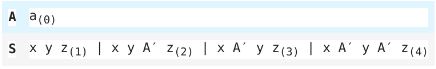
\includegraphics[scale=1]{images/Parsing/esReplace.png}
\end{figure}

A questo punto per sistemarle dobbiamo fare una chiusura, perchè abbiamo prodotto delle epsilon regole, prende tutti i non terminali che non abbimo ancora visto e se quel terminale tra i lati destri di A c'è una epsilon regola faccio il rimpiazzamento e segno che l'ho fatto.
\begin{lstlisting}
@closure
def inline_epsilon_rules(G_seen):
  G, seen = G_seen
  for A in G.N - seen:
    if (epsilon, ) in G.alternatives(A):
      return replace_in_rhs(G, A), seen | {A}
  return G, seen

# esempio d'uso

U = Grammar.from_string("""
S -> A
A -> B C
B -> epsilon
C -> epsilon
""")
U, _ = inline_epsilon_rules((U, set()))

U.P
\end{lstlisting}

\begin{figure}[ht!]
  \centering
  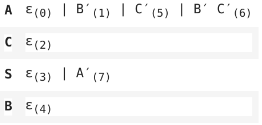
\includegraphics[scale=1]{images/Parsing/esInline.png}
\end{figure}

Osserviamo che questo procedimento non ha tolto le epsilon regole ma le ha messe inline, le mette dove accadevano, quello che succede è che queste regole prima o poi diventano unreachable quindi prima o poi questa regola la toglieremo. L'altro effetto è che solleva la epsilon fino al simbolo distinto, quindi quello che accade è che questo linguaggio potrebbe produrre la parola vuota.
Usando i passi precedenti è semplice arrivare al passo di eliminazione:
\begin{lstlisting}
def eliminate_epsilon_rules(G):
  Gp, _ = inline_epsilon_rules((G, set()))
  prods = set(Gp.P)
  for Ap in Gp.N - G.N:
    A = Ap[:-1]
    for alpha in set(Gp.alternatives(A)) - {(epsilon, )}:
      prods.add(Production(Ap, alpha))
  return Grammar(Gp.N, Gp.T, prods, Gp.S)

# esempio d'uso (fig. 4.10, pag. 120)

U = Grammar.from_string("""
S -> L a M
L -> L M 
L -> epsilon
M -> M M
M -> epsilon
""")

eliminate_epsilon_rules(U).P
\end{lstlisting}

\begin{figure}[ht!]
  \centering
  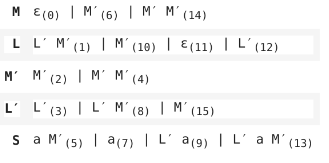
\includegraphics[scale=1]{images/Parsing/esEliminateEpsilon.png}
\end{figure}

\subsection{Eliminazione delle unit rules}
Le regole unitarie sono quelle della forma A -> B, cioè una variabile che deriva un'altra variabile. In questo caso mi aspetto anche che ci sia una C che deriva B e A che deriva qualcos'altro che non è B. Quello che si fa è in tutte le regole dove c'è la A ci metto tutte le alternative. Dato B -> $\omega_1 | \omega_2$ e $C -> \alpha A B$ posso fare $C -> \alpha \omega_1 | \alpha \omega_2$. Faccio questa sostituzione a meno che non mi trovi nel caso del loop $B -> B$.
Prendo tutte le produzioni che sono lunghe 1, le spacco, dico che A produce B, se B è un non terminale prendo le produzioni e faccio l'inline, faccio in modo che A produca tutte le produzioni di B e poi elimino A produce B:
\begin{lstlisting}
def eliminate_unit_rules(G):
  @closure
  def eliminate(G_seen):
    G, seen = G_seen
    for P in set(filter(Production.such_that(rhs_len = 1), G.P)) - seen:
      A, (B, ) = P
      if B in G.N:
        prods = (set(G.P) | {Production(A, alpha) for alpha in G.alternatives(B)}) - {P}
        return Grammar(G.N, G.T, prods, G.S), seen | {P}
    return G, seen
  return eliminate((G, set()))[0]

# esempio d'uso

U = Grammar.from_string("""
S -> A
A -> B
B -> A | b
""")

eliminate_unit_rules(U).P
\end{lstlisting}

Notiamo che questo porta ad avere una grammatica con delle cose irraggiungibili (dopo che elminiamo le epsilon regole e i non unitari). Se voglio fare pulizia uso la tecnica dell'altra volta, applico il metodo remove\_unproductive\_unreachable, ma ancora non è quello da cui siamo partiti perchè ad esempio ci sono dei non terminali oppure delle cose lunghe 3.
Ci rimangono due passaggi:
\begin{enumerate}
    \item Eliminare i non solitari: $A -> \alpha a \beta$. dove alpha e beta non sono terminali
    \item Eliminare le produzioni più lunghe di 2
\end{enumerate}

\subsection{Eliminazione i non solitari}
Un solitario e' un simbolo non terminale se esiste almento una derivazione in cui appare, contribuendo alla produzione di stringhe terminali. 
Per ogni solitario che trovo in giro produco una regola unitaria lunga 1 e sostituisco secco, non ho bisogno neanche di fare le chiusure, cerco le produzioni A B e cerco nel lato destro e guardo cosa sono, se sono dei non terminali li lascio come sono, se sono dei terminali li sostituisco con N e la letterina, dopo di che sostitusico la produzione $Na -> a$ ad esempio:
\begin{lstlisting}
def transform_nonsolitary(G):
  prods = set()
  for A, alpha in G.P:
    prods.add(Production(A, [f'N{x}' if x in G.T else x for x in alpha] if len(alpha) > 1 else alpha))
    prods |= {Production(f'N{x}', (x, )) for x in alpha if x in G.T and len(alpha) > 1}
  return Grammar(G.N | {A for A, alpha in prods}, G.T, prods, G.S)

U = Grammar.from_string("""
S -> x S y S x
""")

transform_nonsolitary(U).P

Ny Y(0)
Nx X(1)
S Nx S Ny S Nx
\end{lstlisting}

Non e' sempre cosi' facile, per le produzioni lunghe faccio produrre ad un primo pezzo A1, x1, x2 poi ad un secondo pezzo A2 faccio produrre A1 x2, così via fino in findo dove avrò A produce A3 x7, partendo da una produzione $A -> x1 x2 x3 x4 x5 x6 x7$:
\begin{lstlisting}
def make_binary(G):
  prods = set()
  for A, alpha in G.P:
    if len(alpha) > 2:
      Ai = f'{A}{1}'
      prods.add(Production(Ai, alpha[:2]))
      for i, Xi in enumerate(alpha[2:-1], 2):
          prods.add(Production(f'{A}{i}', (Ai, Xi)))
          Ai = f'{A}{i}'
      prods.add(Production(A, (Ai, alpha[-1])))
    else:
      prods.add(Production(A, alpha))
  return Grammar(G.N | {A for A, alpha in prods}, G.T, prods, G.S)
\end{lstlisting} 

Ora dobbiamo ricostruire l'albero di parsing, ci verrà più facile rispetto a fare una trasformazione di alberi sostituendo la tabella CYK qualcos'altro.

\subsection{Costruzione albero parsing left-most}
Dato un certo non terminale ci diamo come obiettivo costruire un fattore di una parola di input che partiva da una certa posizione con una certa lunghezza.
Se la lunghezza è 1 devo andare a cercare una produzione della forma X i -1, questa cosa funziona perchè la tabella è costruita correttamente. Se andiamo a riprenderlo è uguale a fake parse, non metto gli alberi ma metto le produzioni. Quindi per ottenere una derivazione leftmost ragioniamo come per la funzione fake\_parse ma invece di restituire un albero restituiamo l'indice della produzione in gioco:
\begin{lstlisting}
 def get_leftmost_prods(G, R, INPUT):
  def prods(X, i, l):
    if l == 1:
      return [G.P.index(Production(X, (INPUT[i - 1],)))]
    for A, (B, C) in filter(Production.such_that(lhs = X, rhs_len = 2), G.P):
      for k in range(1, l):
        if B in R[i, k] and C in R[i + k, l - k]:
          return [G.P.index(Production(A, (B, C)))] + prods(B, i, k) + prods(C, i + k, l - k)
  return prods(G.S, 1, len(INPUT))     

leftmost_prods = get_leftmost_prods(G_cnf, R, INPUT)
leftmost_prods
[28, 31, 9, 12, 7, 37, 20, 11, 1, 6, 32, 15, 30]
d = Derivation(G_cnf).leftmost(leftmost_prods)
ProductionGraph(d)
\end{lstlisting}

\begin{figure}[ht!]
  \centering
  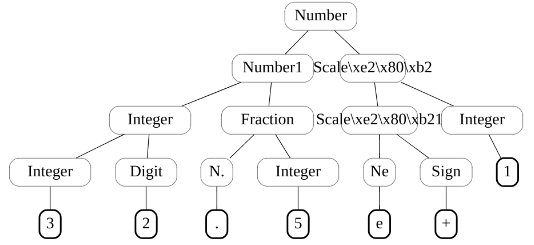
\includegraphics[scale=1]{images/Parsing/derivazioneLeftmostCMK.png}
\end{figure}

Bisogna considerare anche cosa succede nelle produzioni non binarie, mi piacerebbe avere una funzione derives che prende una sequenza di simboli, una i e una l e restituisce una serie di lunghezze ln tale per cui l0 è la lunghezza derivata da w0 input i + i + l0. Per farlo dovrà fare una ricorsione sulla tabella.
Mi sono perso mannaggia a me, ma era abbastanza inseguibile, prova a vedere dal libro.

\section{Parsing Top-down, caso generale}
Andiamo dal basso verso l'alto, da sinistra a destra senza occuparci particolarmente delle grammatiche.
Cominciamo ragionando sull'automa, abbiamo un nastro che legge da sinistra verso destra e teniamo una pila in cui manteniamo lo stato del parsing e poi il controllo che facendo uso del nastro che legge in modo direzionale e della pila deve riuscire a risolvere il problema del riconoscimento, anzi meglio dovrebbe sputare l'albero di parsing della parola.

Facciamo un'assunzione sulla forma della grammatica che ci viene comoda per definire il controllo, una volta definito il controllo riusciremo a rilassare questa assunzione.

Proviamo a ragionare su questa grammatica:

\begin{lstlisting}
    S -> aBC
    A -> aB | b
    C -> a

    w = aaba
\end{lstlisting}

Il riconoscimento è molto semplice se ci basiamo sulle produzioni, partendo da S vediamo che produce a, ma cosa ci facciamo della B e della C? adesso il punto cruciale dato che voglio una left-most mi occupo di B, che a questo punto posso solo sostituire con la sua produzione ottenendo aB, a questo punto sempre dato che voglio una left-most devo occuparmi della nuova B generata e non ho scelta se non sostituirla con aB, vado avanti così fino alla fine.
%metti esempio derivazione

L'idea è che inizio con una pila sulla quale ho il simbolo di partenza S, a questo punto applico la regola 0 e cancello la S e metto sulla pila in ordine inverso le produzioni che ho appena applicato (ci metto solo i non terminali). A questo punto la pila contiene CB, tolgo la B dalla cima della pila, con la sua produzione mi mangio la seconda a e metto sulla pila la B che resta dalla produzione di B, vado avanti così fino a che non ho più nulla da mangiare (mangiare sono i terminali minuscoli che vogliamo trovare che compongono la parola) e la pila è vuota.

Il controllo che abbiamo possiamo considerarlo come una tabella che ha il top della pila, la head della parola e lo stack che contiene i non terminali che sono stati messi in pila:
\begin{table}
    \centering
    \begin{tabular}{|c|c|c|}
        \hline
        \textbf{PILA} & \textbf{HEAD} & \textbf{STACK} \\
        \hline
        S & a & BC \\
        B & a & B \\
        B & b & B \\
        C & a & B \\
        \hline
    \end{tabular}
    \caption{Tabella di controllo del parser top-down}
\end{table}

Mi voglio tenere anche la storia della derivazioni. Nella funzione della libreria mettiamo un \# alla fine della pila e della parola per sapere quando fermarci, ci feriamo quando arriviamo al cancelletto della pila e al cancelletto della parola. Questa descrizione istantanea può evolvere attraverso un passo di predizione, ho decisio che produzione applicare e quindi il passo di predizione ci porta ad avere tolto il lato sininistro della produzione dalla pila e messo il lato destro della produzione sulla pila.
Posso semplificare applicando due nuove regole:
\begin{enumerate}
    \item $(x, x) \rightarrow //$ passo di predizione
    \item $(A, ) \rightarrow \chi \in N$ passo di Match
\end{enumerate}

Quindi a questo punto il controllo o mette una cosa sulla pila oppure toglie dalla pila se sulla cima c'è un non terminale che sta anche sul nastro. Sostanzialmente la testina legge le lettere della parola, il controllo se trova sulla cima della pila un terminale (lettera minuscola) lo consuma e lo toglie dalla pila spostando la testina del nasto a destra, se trova un non terminale lo sostituisce con la produzione e lo mette sulla pila. Se la cima della pila è il cancelletto e la testina è sul cancelletto allora ho finito.

In questo esempio vediamo una simulazione su visite del DAG delle computazioni, in ogni nodo i conserviamo la descrizione istantanea piu' la derivazione che ha condotto a tale derivazione (la grammatica e' quella di prima). Notiamo che all'inizio la pila viene mostrata da sinistra a destra, laa cima della pila e' il carattere piu' a sinistra e che sulla pila all'inizio e' stato aggiunto il simbolo terminale e poi la S e in coda al nastro e' stato aggiunto il simbolo terminale mentre tra parentesi abbiamo il passo di derivazione che ha portato a quella situazione.:
\begin{lstlisting}
i = TopDownInstantaneousDescription(G, 'aaba')

output: (), S#, |aaba#

i = i.predict(G.P[0])
output: (s -> a B C,), aBC#, |aaba#

i = i.match()
output: (S -> a B C,), BC#, a | aba#

i = i.predict(G.P[2])
output: (S -> a B C, B -> a B, B -> b), bC#, aa|ba#

.
.
.

i = i.match()
output: (S -> a B C, B -> a B, B -> b, C -> a), #, aaba|#
\end{lstlisting}

Notiamo che i passi raccolti (nello stesso ordine di quello con cui sono usati da predict) sono quelli di una derivazione leftmost:

\begin{figure}[ht!]
  \centering
  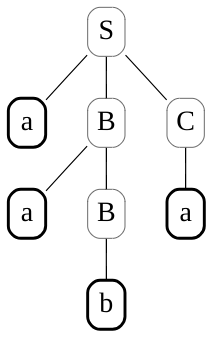
\includegraphics[scale=0.5]{images/Parsing/derivazioneLeftmostTopDown.png}
\end{figure}

\subsection{Funzione stato prossimo}
Per ora abbiamo visto una grammatica in cui la parte di sinistra non aveva ripetizioni, normalmente potremmo avere una grammatica in cui:
\begin{lstlisting}
    S -> aB | aC
    (S, a) -> aB
    (S, a) -> aC
\end{lstlisting}

E questo produce una situazione di non determinismo. Per risolvere questo problema esistono tecniche teoriche e pratiche. La tecnica teorica è quella di avere un dio che dice ad ogni passo cosa fare, a noi non basta perchè non abbiamo dio direttamente da interrogare.
Possiamo immaginarci un grafo della composizione istantanea in cui i nodi sono le istantanee sulla pila e gli archi sono i passi di predizione e match. Nel caso di non determinismo abbiamo più archi che partono dallo stesso nodo (perchè sono tutte le possibili produzioni che posso applicare). Questa la chiamiamo funzione a stato prossimo, quindi partnendo dalla pila e dal nastro (con la parola) possiamo costruire questo grafo che poi possiamo visitare. In questo grafo troviamo dei nodi morti (dead end) che non portano a nulla e dei nodi che portano a qualcosa.
Devo trovare una tecnica di visita che mi porti a trovare i nodi che portano a qualcosa (verdi), la prima idea è una visita in ampiezza in cui posso anche fermarmi quando trovo il primo nodo verde.
Il secondo aspetto è che potrei avere delle situazioni in cui arrivo allo stesso nodo ma in modi diversi, sempre il problema dell'ambiguità. Ad esempio in questa grammatica:
\begin{lstlisting}
    S -> A | B
    A -> a | Ae
\end{lstlisting}

Quello che faccio è considerare uguali due istantanee se la pila e la testina sono uguali (non mi interessa come arrivo a quella situazione), $i = i^{'} PILA; TESTINA$. 

Cominciamo ad immaginare come produrre questo grafo, concentriamoci sulla visita in ampiezza.
La cosa più facile è costruire una funzione stato prossimo, voglio costruire una funzione che data una situazione istantanea mi restituisca tutti gli archi. Mi tengo insieme a questi archi un'etichetta che mi dice se questo arco deriva da un passo di produzione o di match.

\begin{lstlisting}
# restituisce un elenco di coppie (s, tid) 
# dove s e 'match', o la str(P) dove P e una produzione di G e bid e una TopDownInstantaneousDescription
# ottenuta applicando il match o la predizione secondo P a curr

def next_instdescrs(instdescr):
  if instdescr.is_done(): return []
  G = instdescr.G
  top = instdescr.top()
  if top in G.T:
    return [('match', instdescr.match())] if top == instdescr.head() else []
  else:
    return [(str(P), instdescr.predict(P)) for P in filter(Production.such_that(lhs = top), G.P)]
\end{lstlisting}

Come detto la prima cosa che vogliamo fare è una derivazione in ampiezza, metto in una coda i nodi che ho visitato sotto l'assunzione che ho visto il nodo che ha la stessa configurazione di pila e nastro. Il problema se abbiamo ricorsioni è che potremmo andare all'infinito perchè il grafo diventerebbe infinito, quindi ci fermiamo al primo stato istantaneo buono (il verde) questo e' quello che fa il parametro first\_only.
\begin{lstlisting}
def breadth_first(G, word, verbose = False, first_only = True):
  graph = prepare_graph()
  q = Queue()
  q.enqueue(TopDownInstantaneousDescription(G, word))
  seen = {q.Q[0]}
  derivations = []
  while q:
    if first_only and derivations: break
    if verbose:
      for i in q: print(i)
      print('-' * 60)
    curr = q.dequeue()
    for what, nxt in next_instdescrs(curr):
      graph.edge(curr, nxt, gv_args={'label': what})
      if nxt.is_done(): derivations.append(nxt.steps)
      if not nxt in seen: 
        seen.add(nxt)
        q.enqueue(nxt)  
  return derivations, graph
\end{lstlisting}

Ora usiamo una visita in profondità, modifichiamo il tappo di visita, non mi fermiamo alla prima ma contiamo i passi che faccio, se li supero mi fermo.
\begin{lstlisting}
def depth_first(G, word, verbose = False, max_steps = -1, use_seen = True):
  graph = prepare_graph()
  s = Stack()
  s.push(TopDownInstantaneousDescription(G, word))
  seen = {s.S[0]}
  derivations = []
  steps = 0
  while s:
    if steps > max_steps > -1: break
    steps += 1
    if verbose:
      for i in s: print(i)
      print('-' * 60)
    curr = s.pop()
    for what, nxt in next_instdescrs(curr):
      graph.edge(curr, nxt, gv_args={'label': what})
      if nxt.is_done(): derivations.append(nxt.steps)
      if not nxt in seen: 
        if use_seen: seen.add(nxt)
        s.push(nxt)  
  return derivations, graph
\end{lstlisting}

Con questo nuovo algoritmo notiamo che la coda non contiene più tanti elementi, ma 2/3 alla volta. Vediamo che il grafo scende molto più di prima.

Il problema è proprio la ricorsione, cosa succede se ho regole in cui ho S come ricorsione a sinistra? del tipo:
\begin{lstlisting}
    S -> S a | b
\end{lstlisting}

Questo produce una situazione in cui, anche se ho una parola breve, facendo una visita in ampiezza la parola la trovo, ma se faccio una visita in profondità le derivazioni verdi non le trova, perchè non ha un loop nella pila (trova i rossi quando ritrova stati uguali) la pila aumenta all'infinito e non trova mai la parola.

Un modo per correggere il tiro c'è, in particolare la presenza di epsilon regole è drammatica (la pila aumenta senza consumare il nastro), però se evitiamo le epsilon regole possiamo, data una grammatica monotonica (in cui la forma sentenziale non si può ridurre, per noi è la pila) possiamo fermarci quando la pila è troppo lunga, ad esempio se devo generare pippo e sulla pila ho più di 5 non terminali non posso generare pippo, ma genererò una parola di più di 5 caratteri. Quindi nella visita se mi infilo in una circostanza in cui so che non incontrerò mai un nodo verde allora posso fermarmi.
Allora posso considerare una produzione produttiva se la sua produzione è più corta di quello che resta da mangiare.
\begin{lstlisting}
def next_instdescrs(curr):
  def productive(pair):
    _, instdescr = pair
    return len(instdescr.stack) <= (len(instdescr.tape) - instdescr.head_pos)
  return list(filter(productive, original_next_instdescrs(curr)))
\end{lstlisting}

Considero produttive solo le situazioni in cui sulla pila ho un numero di terminali sensato per la parola che ho da generare. Quindi così anche con una visita in profondità riesco a trovare la parola. Notiamo che con la perdita delle epsioln regole perdiamo la possibilità di avere una produzione infinita.

Una cosa carina è che potremmo cambiare la scelta di dove andare solamente basandoci sul nostro passato (se sono arrivato allo stesso punto), posso vedere di togliere questa condizione, ovvero non mi pongo il problema di arrivare in un posto nello stesso modo (non mi interessa il passato). Ovvero se introduciamo l'ambiguità quello che troveremo e' alla fine sempre tutte le derivazioni con la differenza che potremmo avere archi doppi allo stesso nodo, questo perche' potrei arrivare a quel nodo ma con storie diverse quindi togliendo la condizione di uguaglianza tra istantanee potrei avere piu' archi che arrivano allo stesso nodo.

\section{Parsing Ricorsivo Discendente}

\subsection{Eliminare Ricorsione a Sinistra}
Eliminare la ricorsione è una cosa molto comoda anche per poter usare alcuni parser generator che funzionano solo se non c'è la ricorsione quindi è un trucco su cui vale la pena fare un discorso.

Il caso più elementare, se abbiamo un terminale che ha una ricorsione a sinistra questa cosa vorrebbe generare un ciclo, una lista finita di elementi:
\[
A \rightarrow A \alpha_1 | A\alpha_2 ... | \beta_1 | \beta_2 ...
\]

Quindi quello che faremo è introdurre dei nuovi terminali, la testa si occupa di generare i beta, poi similmente si definisce un A di coda che permette di ottenere gli alpha:
\[
A_H \rightarrow \beta_1 | \beta_2 ...
B_T \rightarrow \alpha_1 | \alpha_2 ...
\]

Poi in realtà per generare la lista devo riportare la ricorsione, la spostiamo a destra inserendo un nuovo terminale:
\[
A_{TS} \rightarrow A_T A_{TS}
\]

Dopo di che posso generare uno dei simboli A:
\[
A \rightarrow A_H A_{TS} | A_H
\]

Abbiamo risolto la ricorsione diretta ma manca quella indiretta, una cosa del genere:
\[
A \rightarrow B \alpha
B \rightarrow C \gamma
C \rightarrow A \beta
\]

L'idea in questo caso è ancora strutturalmente semplice. Un modo semplice per risolvere il problema sarebbe quello di ordinare i non terminali, se potessi chiamarli:
\[
A_1 < A_2 < ... < A_n
\]

Il problema di questo caso è che parto da un non terminale e torno allo stesso. Quello che voglio riscrivere tutte le produzioni per cui quelle in cui non c'è un non terminale come primo simbolo deve essere minore di quello che c'è a destra (voglio evitare catene):
\[
A_i \rightarrow A_j \alpha i < j
\]

Il procedimento è iterativo e si parte con $i = 1$, in questo caso non voglio avere cose della ricorsione diretta $A_1 \rightarrow A_1 \alpha_1 | \alpha_2 ...$ quindi lo abbiamo fatto prima possiamo quindi creare una grammatica senza questa ricorsione. Ora passo a $i=2$ e qui avrò cose del genere:
\[
A_2 \rightarrow A_1 \alpha A_2 \alpha A_3 \alpha ...
\]

Prendo questa grammatica e sostituisco gli $A_1$ con quelli che abbiamo sistemato prima. Andando avanti così riusciamo ad avere una grammatica G senza ricorsione a sinistra.

\subsection{Prefix-Free}

Adesso c'è un ulteriore richiesta che è più sottile, vogliamo parlare dei prefix-free, non è possibile avere un prefisso proprio dentro un linguaggio.
Possiamo dire che una grammatica è prefix free se e solo se tutti i non terminali della grammatica sono prefix free, ossia A non deriva mai sia una parola che un suo prefisso. Non è detto che una grammatica si possa trasformare in prefix free, quindi noi lavoreremo sull'ipotesi che la grammatica sia prefix free.

\subsection{Parsing Ricorsivo Discendente}
L'idea è che vorremmo scrivere una funzione parse che prende in input un simbolo x e un pezzo di forma sentenziale w e restituisce una coppia booleano $w^{'}$ tale per cui se per come è fatta la grammtica x effettua il parsing di un prefisso di w allora restituisce true e il pezzo non parsato di w (nel caso in cui x sia un terminale significa che x deve essere la prima lettera di w).

Vogliamo provare a scrivere il parsing per le espressioni più e meno:
\begin{lstlisting}
    E -> E + T | E - T | T
    T -> t
\end{lstlisting}

Partendo da una grammatica ricorsiva così si può trasformare in una grammatica non ricorsiva:
\begin{lstlisting}
"""
E -> Eh Ets | Eh
Eh -> T
Ets -> Et Ets | Et
Et -> + T | - T
T -> t
"""
\end{lstlisting}

Questa grammatica non è prefix free ma noi vogliamo renderla prefix free, in questo caso possiamo mettere un tappo, sostanzialmente vogliamo vedere se dopo Eh mi devo fermare o no, mi fermo se trovo un cancelletto:
\begin{lstlisting}
G = Grammar.from_string("""
E -> Eh Ets | Eh #
Eh -> T
Ets -> Et Ets | Et #
Et -> + T | - T
T -> t
""")
\end{lstlisting}

Possiamo ragionare per casi, trattando a parte il caso dei non terminali e poi ogni terminale a parte (una sorta di switch). I non terminali devo considerarli sulla scorta delle sua alternative(quel non terminale può produrre questo o quello), nel caso di T l'unica cosa che posso fare per dirti se funziona è vedere se t funziona (richiamando il parse)

\begin{lstlisting}
@show_calls(True)
def parse(X, rest):

  if X in G.T:

    if rest and rest[0] == X: return True, rest[1:]
  elif X == 'T': # T -> t

    return parse('t', rest)

  elif X == 'Eh': # Eh -> T

    return parse('T', rest)

  elif X == 'Et': # Et -> + T | - T

    s, r = parse('+', rest)
    if s: return parse('T', r)
    s, r = parse('-', rest)
    if s: return parse('T', r)

  elif X == 'Ets': # Ets -> Et Ets | Et #

    s0, r0 = parse('Et', rest)
    if s0:
      s1, r1 = parse('#', r0)
      if s1: return True, r1
      return parse('Ets', r0)
  
  elif X == 'E': # E -> Eh Ets | Eh #

    s0, r0 = parse('Eh', rest)
    if s0:
      s1, r1 = parse('#', r0)
      if s1: return True, r1
      return parse('Ets', r0)

  return False, rest
\end{lstlisting}

Bello però noi vogliamo l'albero di parsing, modifichiamo la funzione affinchè ritorni anche i passi left-most con cui x produce il prefisso (lo produce usando regola n):
\begin{lstlisting}
# ora parse restituisce: succ, rest, steps

@show_calls(True)
def parse(X, rest): 

  if X in G.T:

    if rest and rest[0] == X: return True, rest[1:], None

  elif X == 'T':

    s, r, _ = parse('t', rest)
    if s: return True, r, [7]

  elif X == 'Eh':

    s, r, p = parse('T', rest)
    if s: return True, r, [2] + p

  elif X == 'Et':

    s, r, _ = parse('+', rest)
    if s:
      s, r, p = parse('T', r)
      if s: return True, r, [5] + p
    s, r, _ = parse('-', rest)
    if s: 
      s, r, p = parse('T', r)
      if s: return True, r, [6] + p

  elif X == 'Ets':

    s0, r0, p0 = parse('Et', rest)
    if s0:
      s1, r1, _ = parse('#', r0)
      if s1: return True, r1, [4] + p0
      s2, r2, p2 = parse('Ets', r0)
      if s2: return True, r2, [3] + p0 + p2

  elif X == 'E':

    s0, r0, p0 = parse('Eh', rest)
    if s0:
      s1, r1, _ = parse('#', r0)
      if s1: return True, r1, [1] + p0
      s2, r2, p2 = parse('Ets', r0)
      if s2: return True, r2, [0] + p0 + p2

  return False, rest, []
\end{lstlisting}

\subsection{Generazione automatica del parser}

Non è così impensabile partire da una grammatica G e fare un programma che produce la funzione parse, perchè lo abbiamo fatto applicando solamente un pattern (gli if della soluzione sono prodotti, uno per ciascun simbolo, considerando in sequenza le possibili alternative (i lati destri delle produzioni) e restituendo successo al primo tentativo valido), quindi quello che vlgliamo fare è trovare il modo di creare una funzione parse che funziona per una grammatica. Questa cosa si chiama parser generator.

Un esempio e' il simbolo Ets le cui due alternative sono Et Ets e Et \# ... supponiamo di scaricarne la soluzione a due funzioni denominate Ets\_alt0 e Ets\_alt1:
\begin{lstlisting}
def parse(X, rest):

  # ...

  if X == 'Ets':
    succ_alt, rest_alt = Ets_alt0(rest)
    if succ_alt: return True, rest_alt
    succ_alt, rest_alt = Ets_alt1(rest)
    if succ_alt: return True, rest_alt
    return False, rest

  # ...

def Ets_alt0(rest):
  succ, rest = parse('Et', rest)
  if not succ: return False, rest
  succ, rest = parse('Ets', rest)
  if not succ: return False, rest
  return True, rest

def Ets_alt1(rest):
    succ, rest = parse('Et', rest)
    if not succ: return False, rest
    succ, rest = parse('#', rest)
    if not succ: return False, rest
    return True, rest
\end{lstlisting}

Quello che facciamo in generale è che ogni volta che un non terminale aveva delle alternative le abbiamo eseguite in cascata invocando una certa funzione che usava quella alternativa, se restitueva true tornavamo altrimenti andavamo nell'else.
Ci servono due funziononi di utilita': la prima per indentare un blocco di testo al livello di indentazione specificato e la seconda per tradurre il codice sorgente di una funzione Python di nome parse in codice eseguibile:
\begin{lstlisting}
def indent_at(level, source):
  return indent(dedent(source), '  ' * level).strip('\n')

def make_parse(source):
  glb = {'show_calls': show_calls}
  exec(source, glb)
  return glb['parse']
\end{lstlisting}
Siamo pronti per procedere, useremo le f-stringhe per maggior compattezza:
\begin{lstlisting}
def make_parse_source(G):

  # prima le definizioni delle funzioni A_altN

  defs = []
  for A in G.N:
    for n, a in enumerate(G.alternatives(A)):
      # la funzione "{A}_alt{n}"
      defs.append(f'def {A}_alt{n}(rest):')
      for X in a: 
        # una coppia di linee per ogni simbolo
        defs.append(indent_at(1, f'''
          succ, rest = parse('{X}', rest)
          if not succ: return False, rest
        '''))
      defs.append(indent_at(1,'return True, rest'))

  # poi gli if, uno per terminale

  ifs = []
  for A in G.N:
    # l'if "X == '{A}'"
    ifs.append(f"if X == '{A}':")
    for n, _ in enumerate(G.alternatives(A)): 
      # una coppia di linee, una per alternativa
      ifs.append(indent_at(1, f'''
        succ_alt, rest_alt = {A}_alt{n}(rest)
        if succ_alt: return True, rest_alt
      '''))
    ifs.append(indent_at(1,'return False, rest'))

  # in fine i terminali

  ifs.append(indent_at(0, f'''
    if X in {G.T}:
      if rest and rest[0] == X: return True, rest[1:]
      return False, rest
  '''))

  # e ora mettiamo tutto assieme 

  parse = '\n'.join((
    indent_at(0, '''
      @show_calls(True)
      def parse(X, rest):
    '''), 
    indent_at(1, '\n'.join(defs)), 
    indent_at(1, '\n'.join(ifs))
  ))

  return parse
\end{lstlisting}

Faremo per tutti i non terminali genereremo una serie di or e poi una funzione specifica che fa la concatenazione. L'unica cosa che ci serve è mettere a posto l'indentazione.
Python ci permette, data una stringa sorgente renderla eseguibile, prende un sorgente di una parse e restituisce una funzione che fa il parsing (reflection di python).
Se generaiamo e stampiamo il sorgente otteniamo questo:
\begin{lstlisting}
source = make_parse_source(G) # G e la grammatica prefix-free dell'inizio
print(source)

@show_calls(True)
def parse(X, rest):
  def Ets_alt0(rest):
    succ, rest = parse('Et', rest)
    if not succ: return False, rest
    succ, rest = parse('Ets', rest)
    if not succ: return False, rest
    return True, rest
  def Ets_alt1(rest):
    succ, rest = parse('Et', rest)
    if not succ: return False, rest
    succ, rest = parse('#', rest)
    if not succ: return False, rest
    return True, rest
  def E_alt0(rest):
    succ, rest = parse('Eh', rest)
    if not succ: return False, rest
    succ, rest = parse('Ets', rest)
    if not succ: return False, rest
    return True, rest
  def E_alt1(rest):
    succ, rest = parse('Eh', rest)
    if not succ: return False, rest
    succ, rest = parse('#', rest)
    if not succ: return False, rest
    return True, rest
  def Et_alt0(rest):
    succ, rest = parse('+', rest)
    if not succ: return False, rest
    succ, rest = parse('T', rest)
    if not succ: return False, rest
    return True, rest
  def Et_alt1(rest):
    succ, rest = parse('-', rest)
    if not succ: return False, rest
    succ, rest = parse('T', rest)
    if not succ: return False, rest
    return True, rest
  def Eh_alt0(rest):
    succ, rest = parse('T', rest)
    if not succ: return False, rest
    return True, rest
  def T_alt0(rest):
    succ, rest = parse('t', rest)
    if not succ: return False, rest
    return True, rest
  if X == 'Ets':
    succ_alt, rest_alt = Ets_alt0(rest)
    if succ_alt: return True, rest_alt
    succ_alt, rest_alt = Ets_alt1(rest)
    if succ_alt: return True, rest_alt
    return False, rest
  if X == 'E':
    succ_alt, rest_alt = E_alt0(rest)
    if succ_alt: return True, rest_alt
    succ_alt, rest_alt = E_alt1(rest)
    if succ_alt: return True, rest_alt
    return False, rest
  if X == 'Et':
    succ_alt, rest_alt = Et_alt0(rest)
    if succ_alt: return True, rest_alt
    succ_alt, rest_alt = Et_alt1(rest)
    if succ_alt: return True, rest_alt
    return False, rest
  if X == 'Eh':
    succ_alt, rest_alt = Eh_alt0(rest)
    if succ_alt: return True, rest_alt
    return False, rest
  if X == 'T':
    succ_alt, rest_alt = T_alt0(rest)
    if succ_alt: return True, rest_alt
    return False, rest
  if X in frozenset({'+', '-', 't', '#'}):
    if rest and rest[0] == X: return True, rest[1:]
    return False, rest
\end{lstlisting}

Notiamo che è una ricorsione con backtracking, non scendo all'infinito ma mi fermo prima in alcuni casi.

La cosa drammatica di questo parser è che se ho due alternative tengo sempre buona la prima, ma se il linguaggio non è context free potrei entrare dentro il prefisso e poi dentro li andrei avanti all'infinito. In questo esempio vediamo che parsando alla fine ottengo true con una lista non vuota, quindi sembrerebbe che non ha parsato:
\begin{lstlisting}
# una grammatica non prefix-free (L = {a, ab})

G = Grammar.from_string("""
S -> a | a b
""")

# costruiamo il parser e tentiamo il parse

source = make_parse_source(G)
parse = make_parse(source)
parse('S', 'ab')

(True, 'b') 
\end{lstlisting}

Il problema che non è questa la strada, di fronte ad una disgiunzione $A -> B | C$ non posso prendere per buona solo la produzione B ed ignorare il fatto che potrebbe produrre anche C (che potrebbe essere meglio), ed è ovviamente un grande limite. Quello che si potrebbe fare è avere un parsing con le continuazioni, sostanzialmetne restituisco nel parse anche una funzione che prova tutte le alternative. Il problema di questa cosa è che si risolve il problema ma non è più lineare, perchè fa tutte le alternative.

In buona sostanza avere un parsing ricorsivo discendente è fighissimo perchè è lineare, semplice da implementare e permette di avere già in mano l'interprete. Ad esempio il parsing ricorsivo discendente è quello di Python.
Forse se stiamo costruendo il nostro DSL, con delle regole semplici (comandare drone, irrigazione ...), possiamo permetterci di avere un parsing ricorsivo discendente, ma se vogliamo fare un parser generico per un linguaggio generico non possiamo permetterci di avere un parsing ricorsivo discendente.

\section{Parsing Bottom-Up}
La realizzazione di parsing bottom up veniva più facile negli anni 70 infatti si e' partiti da questo tipo di parser, ragionare su parsing concreti per le grammatiche context-free deterministiche era più facile. Aggiustare una grammatica per farlo funzionare in questo contesto è più difficile questo perchè funziona al contrario rispetto agli altri parser.
Interessante perchè è a livello storico è il primo parsing che si occupa di un grosso numero di grammatiche in tempo lineare ma è doloroso perchè richiede uno sforzo al progettista di grammatiche.

Abbiamo sempre in mente la pila (che contiene i simbli), il nastro e il controllo. L'idea e' mettere sopra il nastro degli alberi, costruire degli alberi che rappresentano delle porzioni della parola (le derivazioni) e li uniscono verso l'alto per avere l'albero di derivazione costruito dal fondo all'alto. Quindi il punto cruciale di questo algoritmo è cominciare a guardare la base e poi la foresta che mi sono costruito sul nastro, quindi sulla pila devo tenere oltre ai tereminali e non terminali devo tenere anche questi alberi.
Allora la cosa più comoda da considerare è che di fatto nella pila voglio tenere le cime degli alberi della foresta, ma correlata a questa informazione i passi che ho fatto.

\subsection{Shift e Reduce}
Quando vedo un carattere sul nastro posso:
\begin{itemize}
  \item Metterlo sulla cima della pila, facendo uno shift
  \item Riconoscere che sulla pila c'è il contenuto di una regola produttiva, nella grammatica c'era da qualche parte $A \rightarrow CD$ allora potrei togliere dalla pila C e D e mettere A, quindi ho fatto una riduzione (reduce). Da notare che in questo esempio eravamo in una situazione in cui sulla pila c'erano D e C che a loro volta rappresentavano un albero di derivazione.
\end{itemize}

Quindi il controllo cerca regole della grammatica il cui lato destro è l'unione di elementi sulla pila. Questa configurazone non è proprio un'automa a pila, perchè non guardo solo la cima della pila, ma spio tutta la pila. Il che sembrerebbe suggerire che questa è una macchina ti Touring, ma scopriremo che non è così. Quello che va colto è che è un approccio inerentemente più complesso perchè l'indecisione è più grande, perchè non solo devo decidere in caso di regole multiple cosa fare ma devo anche decidere se fare uno shift o una riduzione e anche nel caso della riduzione devo decidere quale regola applicare.

Adesso come sempre se abbiamo in testa una cosa che non è deterministica non riusiamo nella pratica a trovare la soluzione, mi immagino di avere una forma descrittiva dello stato della computazione (una descrizione che racconta i passi della computazione), produrre una funzione next che dirà data una delle circostante cosa fare (uno shift e quale reduce fare) che mi dirà quali sono le successive istantanee oppure che nessun lato destro della grammatica fa parte della pila (siamo rovinati) o che abbiamo finito il nastro (abbiamo finito di parsare).

A questo punto simulo, parto da uno stadio iniziale e poi con una modalità breadth-first (allargo la vista) o con modalità depth-first (più pericolosa perchè potrei andare giù all'infinito).

Vediamo una grammatica e facciamo un atto di fede in cui la pila è undbound (perchè ci teniamo dentro anche i passi di derivazione):

\begin{lstlisting}
G = Grammar.from_string("""
S -> A C
A -> a b
C -> c
""")

i = BottomUpInstantaneousDescription(G, 'abc')
# (), , |abc

i = i.shift()
display(i, side_by_side(i.stack))
# (), (a), a|bc

i = i.shift()
display(i, side_by_side(i.stack))
# (), (a)(b), ab|c

i = i.reduce(G.P[1])
display(i, side_by_side(i.stack))
# (A -> a b,), (A: (a), (b)), ab|c

. . .

i = i.reduce(G.P[0])
display(i, side_by_side(i.stack))
# (S -> A C, C -> c, A -> a b), (S: (A: (a), (b)), (C: (c))), abc|
\end{lstlisting}

Vediamo che la descrizione istantanea è come l'altra, ho i passi di derivazione, la pila vuota, la testina e il nastro.
A botte di shift e reduce portiamo un po' di simboli sulla pila e quando vedo che sulla pila ci sono delle regole destre della grammatica tolgo quelle teste e ci metto l'albero di derivazione.

Adesso ragioniamo su come fare la funzione next, l'aspetto cruciale è che abbiamo un automa che ha delle primitive che si riflettono sulla sua natura di automa a pila, dopo di che siccome per ogni condizione in cui si trova ho un certo insieme finito di possibilità (non ristretto ad 1) posso fare una simulazione che devo fare con la funzione next.
Il passo di riduzione è più difficile da implementare perchè devo prendere tutto lo stack, corrisponde ad una lettura completa della pila (dal punto di vista di programmazione ad oggetti svelo tutto lo stato dell'oggetto). All'occhio che qui non ci sono le epsilon regole.

\begin{lstlisting}
G = Grammar.from_string('S -> a S b | S a b | a a a')
derivations, graph = breadth_first(G, list('aaaab'), True, False) # raccolgo tutte le derivazioni
\end{lstlisting}

\begin{lstlisting}
# restituisce un elenco di coppie (s, bid) 
# dove s e' 'shift', o la str(P) dove P e' una produzione di G e bid e' una BottomUpInstantaneousDescription
# ottenuta applicando lo shift o la riduzione usando P a curr

def next_instdescrs(curr):

  if curr.is_done(): return []

  instdescrs = []

  # shift
  if curr.head_pos < len(curr.tape): instdescrs.append(('shift', curr.shift()))
  if curr.G.has_epsilon_productions(): instdescrs.append(('e-shift', curr.shift(False)))
 
  # reduce
  tops = tuple(t.root for t in curr.stack)
  for P in filter(Production.such_that(rhs_is_suffix_of = tops), curr.G.P):
    instdescrs.append((str(P), curr.reduce(P)))

  return instdescrs


# una funzione che associa ad ogni descrizione un colore 
# a seconda che sia accettante (verde), o non abbia stati prossimi (rosso)
def node2color(tid):
  return {'color': 'green' if tid.is_done() else 'black' if next_instdescrs(tid) else 'red'}
\end{lstlisting}

Possiamo usare lo stesso codice dell'altra volta per fare la visita in ampiezza, abbiamo visto un esempio data una grammatica con ricorsione a sinistra che produce due derivazioni right-most diverse. Vediamo che come l'altra volta abbiamo il parametro first\_only che ci permette di fermarci alla prima derivazione verde.

\begin{lstlisting}
def breadth_first(G, word, verbose = False, first_only = True):
  graph = ComputationGraph(node2color)
  q = Queue()
  q.enqueue(BottomUpInstantaneousDescription(G, word))
  derivations = []
  while q:
    if first_only and derivations: break
    if verbose:
      for i in q: print(i)
      print('-' * 60)
    curr = q.dequeue()
    for what, nxt in next_instdescrs(curr):
      if nxt.is_done(): derivations.append(nxt.steps)
      if not graph.seen(nxt): 
        q.enqueue(nxt)
      graph.step(curr, nxt, what)
  return derivations, graph
\end{lstlisting}

\begin{figure}[ht!]
  \centering
  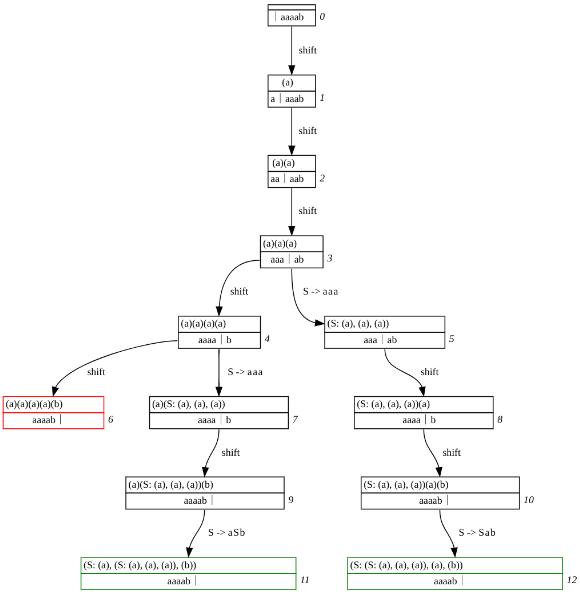
\includegraphics[width=0.8\textwidth]{images/Parsing/bottom_up_breadth.png}
\end{figure}

\newpage

Anche l'approccio con visita in profondità è lo stesso dell'altra volta:
\begin{lstlisting}
def depth_first(G, word, verbose = False, max_steps = -1, use_seen = True):
  graph = ComputationGraph(node2color)
  s = Stack()
  s.push(BottomUpInstantaneousDescription(G, word))
  derivations = []
  steps = 0
  while s:
    if steps > max_steps > -1: break
    steps += 1
    if verbose:
      for i in s: print(i)
      print('-' * 60)
    curr = s.pop()
    for what, nxt in next_instdescrs(curr):
      if nxt.is_done(): derivations.append(nxt.steps)
      if not (use_seen and graph.seen(nxt)): 
        s.push(nxt)  
      graph.step(curr, nxt, what)
  return derivations, graph
\end{lstlisting}

\begin{figure}[ht!]
  \centering
  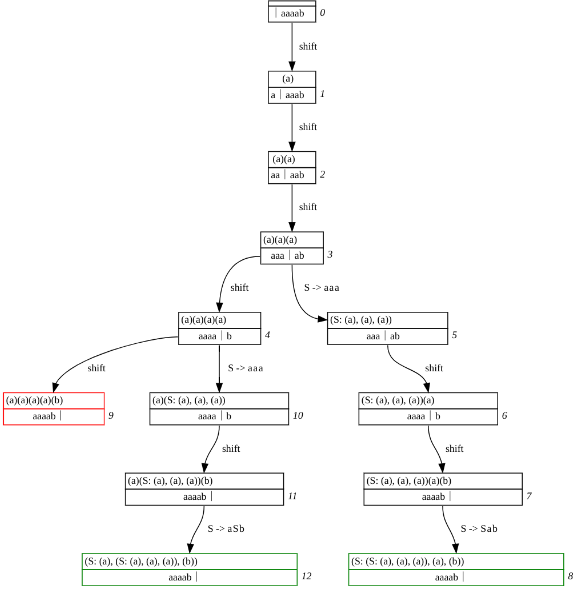
\includegraphics[width=0.8\textwidth]{images/Parsing/bottom_up_depth.png}
\end{figure}



Vediamo un esempio che anche con una grammatica apparentemente elementare ed una stringa corta ha dei problemi non visibili ad occhio nudo, se la proviamo con la visita in profondità è vero che arriva alla soluzione ma sbaglia un sacco di strade.

\begin{lstlisting}
# fig. 7.8, pag. 204

G = Grammar.from_string("""
S -> E
E -> E Q F | F
F -> a
Q -> + | -
""")
\end{lstlisting}

\begin{figure}[ht!]
  \centering
  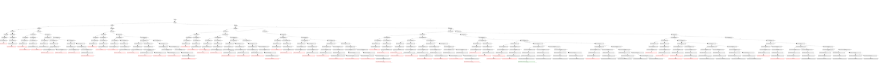
\includegraphics[width=0.8\textwidth]{images/Parsing/bottom_up_realistico.png}
\end{figure}

Questo algoritmo come abbiamo visto è più difficile da ragionarsi sopra in particolare perchè restano due brutte cose da sistemare:
\begin{itemize}
  \item Devo leggere tutta la pila
  \item Devo tenere tutti gli alberi
\end{itemize}

Ma anche supponendo che questi problemi teorici vengano risolti resta il fatto che purtroppo in questo caso le grammatiche che producono il disastro sono molto più difficili da vedere rispetto alle grammatiche che producono il disastro per i parser top down. Esistono strumenti automatici che ci dicono se la grammatica è ambigua o meno per i parser bottom up (LR(0)) ma è comunque doloroso modificare quelle grammatiche malate. Notiamo che TopDown e BottoUp si usano per grammatiche deterministiche e che senza ambiguità hanno costo computazionale $O(n)$, quindi non è un problema di efficienza ma di correttezza. 

Dal lato dei parser Bottom Up ci sarebbe l'algoritmo CYK (che usiamo per le grammatiche generali ed ha costo computazionale $n^3$) bello, che è l'algoritmo di Early che funziona per le grammatiche generali che in caso di non ambiguità per le grammatiche determinstiche (quelle che usiamo TopDown e BottoUP) diventa $O(n)$.

\section{Parsing top-down direzionale deterministico}

Vogliamo metterci nella condizione per cui la cosa che adoperiamo che ha la testina la pila e la parola ad un certo punto vede la cima della pila e la prossima letterla della parola (sotto la testina) il controllo può fare la predizione.
La necessità di seguire tutti i possibili cammini nel grafo che simula la computazione del NPDA deriva dal fatto che per un certo simbolo A in cima alla pila e il primo terminale b sotto la testina, ci sono più produzioni da considerare.
In buona sostanza vogiamo una tabella, che dipende dalla grammatica, che mi dice la corripondenza tra simboli terminali e non terminali e grazie a questa corrispondenza riesco a derivare subito la produzione. Grazie a questa tabella implementare il controllo dell'automa è una banalità, se la cima è un terminale ti dico se c'è un match o no, se la cima è un non terminale ti dico se posso fare una predizione o meno. La magia grande è la tabella che deve funzionare, non deve contenere nessuna produzione se sono in un posto in cui non dovrei essere.

Adesso il punto è come produciamo questa tabella, in realtà la abbiamo già vista, perchè ad un certo punto abbiamo giocato con una grammatica che era così:
\begin{lstlisting}
    S -> aB
    B -> b | aBb
\end{lstlisting}

Funziona bene perchè il primo carattere di ogni produzione è diverso, se sono in una circostanza per cui per ogni possibilità mi porta ad una produzione con il primo carattere diverso allora posso costruire la tabella:
\begin{table}[ht!]
  \centering
  \begin{tabular}{|c|c|c|}
    \hline
    & \textbf{S} & \textbf{B} \\ \hline
    a & S -> ab & B -> b \\ \hline
    b &   & B -> aBb \\ \hline
  \end{tabular}
\end{table}

Queste grammatiche si chiamano SSL(1), dove 1 sta per il numero di simboli che guardiamo dopo la testina.

Per costruire la tabella prendo le produzioni della grammatica, le smonto come lato sinistro e letterina e suffisso e la produco così (se c'è un tentativo di riassegnamento mi avvisa che non è una grammatica che posso trattare), per ogni produzione $A \rightarrow b\delta$ basta considerare il primo simbolo che è terminale e distingue le varie alternative:
\begin{lstlisting}
  def compute_simple_table(G):

  TABLE = Table(2, no_reassign = True) # no_reassign sara chiarito in seguito

  for P in G.P:
    A, (b, +d) = P
    TABLE[A, b] = P

  return TABLE
\end{lstlisting}

Ma se la grammatica non è semplice? nella costruzione della tabella mi avverte che c'è un conflitto (cerca di mettere due entry per la stessa coppia).

Questo modo di costruire i parser è facile ma utile, ad esempio è la notazione prefissa (notazione polacca) che è una notazione che non ha bisogno di parentesi, perchè il parser è in grado di capire la precedenza degli operatori. Ad esempio:
\begin{lstlisting}
G = Grammar.from_string("""
E -> + E E | - E E | * E E | / E E | t
""")
\end{lstlisting}

Questo modo di scrivere le espressioni è molto comodo perchè è immediato parsare le associazioni e le precedenze, ad esempio:
\[\begin{split}
* + 324 \rightarrow (3 + 2) * 4 \\
+ 3 * 2 4 \rightarrow 3 + (2 * 4) 
\end{split}
\]

Questa costrizione è molto stringente, non avere due simboli uguali in due produzionzioni diverse è una cosa che non è sempre possibile, ad esempio vorrebber dire non poter avere if e if else.
Allora una cosa su cui possiamo ragionare è questa, supponiamo di sapere per ogni forma sentenziale qual'è la prima lettera che compare nella derivazione. Mi interessa conoscere data una forma sentenziale i prefissi, di tutte le parole che questa forma sentenziale può produrre quali sono i primi caratteri di queste derivazioni.
Se avessi questa roba qui potrei costruire la tabella in un'altra ottica, metto in tebella le produzioni basandomi sui first, ad esempio se voglio collocare A -> w e so che first(w) = a, b, f allora la tabella sarebbe così:
\begin{table}[ht!]
  \centering
  \begin{tabular}{|c|c|c|}
    \hline
    & \textbf{A} \\ \hline
    a & A -> w\\ \hline
    b & A -> w  \\ \hline
    ... & ... \\ \hline
    f & A -> w \\ \hline
  \end{tabular}
\end{table}

Il first di una forma sentenziale nella forma in cui nessuna delle parti può scomparire (in quanto non ci sono epsilon regole) è il primo simbolo che compare nella derivazione. Nel riempire la tabella posso fare una fattorizzazione, prendo la A e la spacco e poi prendo tutte le lettere che vengono prodotte da B e riempio la tabella:
\begin{lstlisting}
  def compute_table(G):

  TABLE = Table(2, no_reassign = True)

  FIRST = compute_first(G)

  for P in G.P:
    A, (B, *d) = P
    for a in FIRST[B]:
      TABLE[A, a] = P

  return TABLE
\end{lstlisting}

Con questa cosa del first riesco a vedere i conflitti un po' in avanti, un conflitto lo ho quando due produzioni hanno lo stesso first.

Si suggerirebbe un approccio ricorsivo, questo per guardare i first, ricordando che questo è perchè non abbiamo le epsilon regole. Il calcolo di $FIRST(\beta)$ dove si ponda $\beta = C\delta$, può essere semplificato osservando che $FIRST(C\delta) = FIRST(C)$.

\begin{lstlisting}
def compute_first(G):

  def recursive_first(B): # B e G.T | G.N
    return union_of(
      recursive_first(C)
      for C, *d in G.alternatives(B) if B != C # occhio alla ricorsione a sinistra!
    ) if B in G.N else {B}
  
  FIRST = Table(1)
  for X in G.N | G.T: FIRST[X] = recursive_first(X)
      
  return FIRST
\end{lstlisting}

Vediamo un esempio con una garmmatica di un ipotetico sistema esperto nel quale prima si indica un fatto, una sequenza di fatti è una sessione e poi si termina con una domanda:
\begin{lstlisting}
# fig. 8.7, pag. 240

G = Grammar.from_string("""
Session -> Fact Session | Question | ( Session ) Session
Fact -> ! STRING
Question -> ? STRING
""")
\end{lstlisting}

Ricorsivamente possiamo costruire i first, l'idea è che posso usare una regola che ha sessione a sinistra solo se sul nastro vedo uno di questi ?, (), !.
E a questo punto posso costruire la tabella di derivazione, in questo caso non ci sono conflitti e quindi posso costruire la tabella:
\begin{table}[ht!]
 \centering
  \begin{tabular}{|c|c|}
    \hline
    \textbf{Question} & ? \\ \hline
    \textbf{Fact} & ! \\ \hline
    \textbf{Session} & (, !, ? \\ \hline
    \end{tabular} 
\end{table}


L'uso della tabella first mi consente di sapere, non tanto sulla scorta della prima letterina dei lati destri, ma sulla scorta dei first della grammatica (le letterine), se questa tabella non ha conflitti sono a posto, posso chiamare questa roba LL(1) e posso chiamare il parser che funziona:
\begin{enumerate}
  \item first
  \item table if no conflitti:
  \item parser
\end{enumerate}

Abbiamo trovato un parser deterministico lineare, lineare perchè legge ogni lettera una volta sola.

\begin{figure}[ht!]
  \centering
  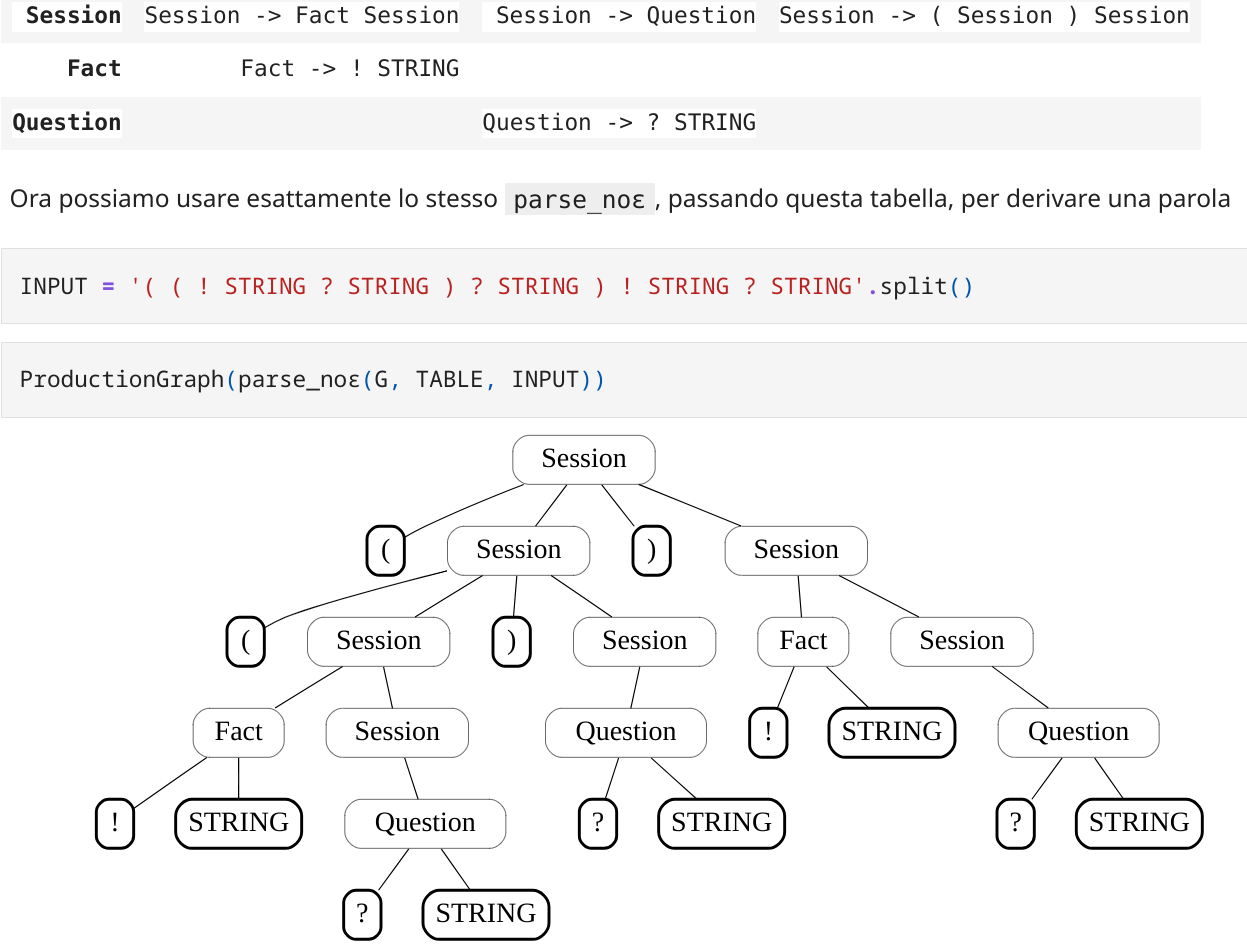
\includegraphics[width=0.8\textwidth]{images/Parsing/tabella_parsing_bottomup.png}
\end{figure}

\subsection{Cosa accade con le epsilon regole}
La presenza delle epsilon regole serve a tradurre meglio l'idea semantica che ho in testa, una sessione di colloquio con il mio sistema esperto è una sequenza di fatti, potenzialmente vuota, seguita da una domanda. Per fare questa roba ho bisogno di fare sparire i fatti, quindi ho bisogno di epsilon regole.

\begin{lstlisting}
# fig. 8.9, pag. 242

G = Grammar.from_string("""
Session -> Facts Question | ( Session ) Session
Facts -> Fact Facts | e
Fact -> ! STRING
Question -> ? STRING
""") 
\end{lstlisting}

Cominciamo col ragionare per gradi, come facciamo la tabella dei first con le epsilon regole? Quello che potrei fare è fare in modo che table sbirci non solo il primo simbolo ma un po' più in giù nella pila, in realtà vedremo che non è necessario, si potrà pre-computare una tabella.

Occuparsi di first in presenza di epsilon regole non è così devastante. Qui non possiamo più fattorizzare il fatto che dobbiamo per forza prendere la prima lettera perchè non sparisce, non è vero, perchè ora può sparire perchè ci sono le epsilon regole. Non vale più $FIRST(B\beta) = FIRST(B)$. Nel caso $FIRST(B\gamma)$:
\begin{itemize}
  \item $\epsilon \not\in FIRST(B)$ allora $FIRST(B\gamma) = FIRST(B)$ sono nel caso di prima
  \item $\epsilon \in FIRST(B)$ allora $FIRST(B\gamma) = (FIRST(B) - \epsilon) + FIRST(\gamma)$, dove gamma sono i simboli che seguono B. Il dramma quindi è che devo capire cosa succede a gamma.
\end{itemize}

Faccio una chiusura, first la computo per tutte le forme sentenziali, quindi una entry della tabella è una tupla:
Riempio mettendo first smontando la forma sentenziale tranne la nullabilità il prefisso e se c'è la nullabilità il suffisso. Consideriamo anche la stringa vuota e il simbolo di fine nastro(per praticità, considereremo anche il caso di suffissi di lunghezza nulla, a cui corrisponderà $\epsilon$). Ad ogni passo la chiusura, per ciascun suffisso $\omega = C\delta$, aggiungerà allàinsieme First($\omega$) i terminali in:
\begin{itemize}
  \item First($C$) se $\epsilon \not\in First(C)$
  \item First($C$) - $\epsilon$ e First($\delta$) se $\epsilon \in First(C)$
\end{itemize}
Per concludere, la seguente implementazione popola FIRST con $FIRST(\omega)$ per tutti i suffissi dei lati destri delle produzioni di G anche qualora siano presneti epsilon regole:
\begin{lstlisting}
 def compute_efirst(G):

  FIRST = Table(1, element = set) # questo significa che gli elementi dell tabella sono insiemi

  # i casi base
  for t in G.T | {e, HASH}: FIRST[(t, )] = {t} # attenzione, gli indici sono forme sentenziali, ossia tuple!

  # il caso di forma sentenziale di lunghezza nulla
  FIRST[tuple()] = {e}

  @closure
  def update_with_suffixes(FIRST):
    for A, a in G.P:
      FIRST[(A, )] |= FIRST[a]
      for o in suffixes(a):
        C, *d = o
        FIRST[o] |= FIRST[(C, )] - {e}
        if e in FIRST[(C, )]: FIRST[o] |= FIRST[d]
    return FIRST

  return update_with_suffixes(FIRST) 
\end{lstlisting}

Chiamando questa funzione sulla nostra grammatica otteniamo:
\begin{table}
  \centering
  \begin{tabular}{c|c}
    \textbf{Session} & \{ $($, !, ? \} \\
    \textbf{Fact} & \{ ! \} \\
    \textbf{Question} & \{ ? \} \\
    \textbf{Facts} & \{ !, e \} \\
    
  \end{tabular}
\end{table}